\documentclass[spanish, a4paper]{article}

\usepackage{ulem}
\hoffset=-2cm \voffset=-2.5cm
\parskip=0.5cm
\topmargin 2cm

\textwidth 16cm
\textheight 24cm

\usepackage{caratula}
\usepackage[spanish]{babel}
\usepackage[utf8]{inputenc}
%\usepackage[latin1]{inputenc}
\usepackage{fancyhdr} %header lindo
\usepackage{listingsutf8}
\usepackage{pdfpages} %incluir pdf


\usepackage{caption}
\usepackage{subcaption}

\providecommand{\keywords}[1]{\textbf{\textit{Palabras Clave ---}} \textit{#1}}

\usepackage{color}

\definecolor{dkgreen}{rgb}{0,0.6,0}
\definecolor{gray}{rgb}{0.5,0.5,0.5}
\definecolor{mauve}{rgb}{0.58,0,0.82}

\lstset{inputencoding=utf8/latin1}
\lstset{
  frame=none,
  xleftmargin=0.1in,
  stepnumber=1,
  numbers=left,
%  numbersep=5pt,
  numberstyle=\ttfamily\tiny\color[gray]{0.3},
  belowcaptionskip=\bigskipamount,
  captionpos=b,
  escapeinside={*'}{'*},
%  language=Prolog,
  tabsize=1,
%  emphstyle={\bf},
%  commentstyle=\it,
%  stringstyle=\mdseries\rmfamily,
  showspaces=false,
  breaklines=true,
%  keywordstyle=\bfseries\rmfamily,
%  columns=flexible,
%  basicstyle=\small\scriptsize,
  basicstyle=\small,
  showstringspaces=false,
  morecomment=[l]\%,
}


\pagestyle{fancy}
\lhead{Teoría de Lenguajes}
\rhead{1C 2017}

\newcommand{\persona}[1]{\underline{#1}}

\begin{document}

\fecha{\today}
\titulo{Teoría de Lenguajes\\\textit{Analizador Sintáctico y Semántico para }$\lambda^{bn}$}
\materia{Grupo: \textit{Ullman, Sethi y los demás}}


\integrante{Gabriel Eric Thibeault}{114/13}{gabriel.eric.thibeault@gmail.com}
\integrante{Gonzalo Ciruelos Rodríguez}{063/14}{gonzalo.ciruelos@gmail.com}
\integrante{Luis Agustín Nieto}{46/01}{lnieto@dc.uba.ar}

\maketitle

%\tableofcontents

\newpage
\section{Introducción}
En el presente trabajo práctico se realiza un analizador sintáctico y semántico para un subconjunto del cálculo lambda tipado sobre booleanos y naturales $\lambda^{bn}$, para dicha implementación se utilizó PLY que es una implementación en Python de las clásicas herramientas \textit{lex} y \textit{yacc}.

El lexer está implementado en \textit{lexer.py}, en el mismo definimos las expresiones regulares y tokens que sirven para definir si cadenas de entrada son o no válidas acorde a la gramática creada. El parser,donde definimos las producciones de nuestra gramática, está implementado en \textit{parser.py}.\\
Se realizaron una serie de test para probar la correcta implementacion del analizador, los mismos se encuentran en \textit{test.py}.

\newpage
\section{Gramática}

La mayor dificultad del trabajo fue armar una gramática que sirviese para para el lenguaje pedido, recordemos que el mismo es:

\begin{verbatim}
M ::= 		x | true | false | if M1 then M2 else M3 | \x:T.M | M1 M2 | 0 | succ(M) 
            | pred(M) | iszero(M)
            
T ::=		Bool | Nat | T1 -> T2            
\end{verbatim}

Luego de varias pruebas se llegó a esta gramática:


$$G = \left<  \{E,S, C, L, T'\}, \{var, true, false, iszero, succ, pred, (, ), 0, Bool, Nat, if, then, else,  \textnormal{\textbackslash}, :, . \}, P, E  \right> \textnormal{, con P:} $$
\begin{eqnarray}
  E & \rightarrow  & S\ L \nonumber \\
    & |            & S  \nonumber \\
  S & \rightarrow  & S\ C \nonumber \\
    & |            & \lambda  \nonumber\\
  C & \rightarrow & (E)  \nonumber\\
    & |           & var  \nonumber\\
    & |           & true  \nonumber\\
    & |           & false  \nonumber\\
    & |           & 0 \nonumber \\
    & |           & iszero(E)  \nonumber\\
    & |           & succ(E)  \nonumber\\
    & |           & pred(E)  \nonumber\\
    & |           & if \: E \: else \: E \: then \: C  \nonumber\\
    L & \rightarrow &  \textnormal{\textbackslash\ V :\ T .\ E } \nonumber\\
  T & \rightarrow & T'\ arrow\ T  \nonumber\\
     & |           & T'  \nonumber\\
  T' & \rightarrow & (T\ arrow\ T')  \nonumber\\
    & |           & Bool  \nonumber\\
     & |           & Nat  \nonumber\\
\end{eqnarray}

Expliquemosla brevemente:
\begin{itemize}
  \item $E$. La idea es que este no terminal represente a todas las expresiones, que o bien pueden ser un $S$, o bien un $S$ aplicado a un $L$.
  \item $S$. Estos terminos seran una lista de aplicaciones a cosas distintas que un L (puede haber un $L$, pero deberá estar entre paréntesis, siguiendo la reducción $S C \rightarrow S (E) \rightarrow S (S L) \rightarrow S (L)$). Este no-terminal nos permite forzar que la aplicación asocie a izquierda (notemos que la producción es recursiva a izquierda).
  \item $C$. Estos serán todos los términos sin paréntesis, excepto los lambda. Necesitamos que los lambda vayan entre paréntesis en general, porque por ejemplo el string $\textbackslash x\ :\ Nat\ .\ x\ y$ no queda claro si es una función aplicada a $y$, o si $x\ y$ es el cuerpo de la abtracción.
  \item $L$. Básicamente las abstracciones lambda.
  \item $T$. Como los tipos flecha asocian a derecha ($Nat \rightarrow Nat \rightarrow Nat$ es $Nat \rightarrow (Nat \rightarrow Nat)$), necesitamos tener dos no terminales para que la grámatica no nos quede ambigua.
  \item $T'$. Los tipos de la derecha de una flecha tienen que, o bien ser un tipo flecha entre paréntesis, o bien ser tipos básicos.
\end{itemize}

Veamos además las expresiones regulares de cada token:
\begin{itemize}
  \item $var$. ``[abcjxyz]'', o sea cualquier letra del conjunto ${a,b,c,j,x,y,z}$, para tener una cantidad suficiente de variables, pero necesitamos prohibir ciertos nombres (por ejemplo ``i'', ``e''), para que no haya conflictos en el parser, porque colisionarian con las sentencias como ``else'' o ``if''.
  \item $arrow$. `` $- >$ ''.
  \item Todas el resto la expresión regular es igual al nombre del token.
\end{itemize}

\newpage
\section{Código}
\subsection{Explicación}
En el código basicamente tenemos una clase para cada tipo de término. Todas estas clases son polimorficas y saben responder los mismos mensajes (evaluate, dame tu tipo, etc). La idea es que el parseo nos devuelva un árbol de todas estas clases, y simplemente le pidamos el valor y el tipo a la raiz, que se ocupará de hacer todas las  llamadas necesarias a sus hijos, y así sucesivamente.

O sea, lo que sucede es que al terminar de parsear tenemos el \textit{AST} de la cadena, y luego la evaluamos siguiendo las reglas del cálculo lambda.

Un paso intermedio no menor (luego de obtener el \textit{AST} pero antes de evaluar) es que le asignamos ``contextos'' a todos los subtérminos de la cadena. Por ejemplo, en la cadena ``(\textbackslash x\ :\ Nat\ .\ x)'', nos gustaría que la clase que representara a la $x$ del cuerpo de la abstracción supiera que esa $x$ tiene tipo $Nat$.

Esto lo logramos con una función llamada ``add\_judgement'', que simplemente lo que hace es tomar el contexto de un término, y pasárselo a todos sus hijos. Además, si el término es un lambda, le va a pasar a los hijos su contexto sumandole un juicio que dice que el parámetro tiene el tipo dado.

Luego, antes de evaluar el \textit{AST}, necesitamos propagar todos estos valores hacia abajo. Logramos esto haciendo una llamada al ``add\_judgement'' de la raíz con valores dummy.

\subsubsection{Conflicto}

En las reglas de los tipos ($T \rightarrow T' -> T$), PLY nos decía que había un conflicto. Esto se soluciona de forma tan fácil como indicarle que la flecha asocia a derecha. Sin embargo, en algunas versiones de PLY no parecía tomar este comando e igualmente salía el Warning, pero lo resolvía de la forma correcta.

\subsection{Uso y Tests}
Para poder ejecutar el código necesitamos instalar varias dependencias, como utilizamos de base el código del taller de \textbf{PLY} usamos el mismo archivo \verb|requirements.txt|, la única diferencia con el taller es que el trabajo está implementado en Python3 por lo que tenemos que usar \textit{pip3} en lugar de \textit{pip}.

\verb| pip3 install -r requirements.txt |

El comando para evaluar expresiones es \textbf{CLambda} y su sintaxis es \verb|./CLambda [EXPRESION]|.\\
Si la expresión es correcta debe devolver su evaluación, caso contrario devuelve un mensaje de error detallando que fue lo que pasó, por ejemplo:

\begin{verbatim}
tlen-tp1$ ./CLambda.py '(\x:Nat. if iszero(x) then succ(x) else pred(x)) 0'
1  :  Nat
\end{verbatim}

O si queremos ver un error de tipado:

\begin{verbatim}
tlen-tp1$ ./CLambda.py '(\x:Nat. if iszero(x) then succ(x) else true) 0'
Ilegal: distintos tipos en el cuerpo del if: 1 y true tienen distintos tipos (Nat y 
Bool respectivamente).
\end{verbatim}

Para testar el correcto funcionamiento de la implementación se armaron varios casos de test dentro del archivo \textit{test.py}, en el mismo se define la expresion el resultado y el tipo esperado de la evaluación. Se hicieron tanto casos satisfactorios como casos de evaluaciones fallidas.\\
Para probarlo solo tenemos que ejecutarlo:


\begin{verbatim}
tlen-tp1$ ./tests.py 
PASSED 0
PASSED true
PASSED if true then 0 else false
PASSED \x:Bool.if x then false else true
PASSED \x:Nat.succ(0)
PASSED \z:Nat.z
PASSED (\x:Bool.succ(x)) true
PASSED succ(succ(succ(0)))
PASSED x
PASSED succ(succ(pred(0)))
PASSED 0 0
PASSED \x:Nat->Nat.\y:Nat.(\z:Bool.if z then x y else 0)
PASSED (\x:Nat->Nat.\y:Nat.(\z:Bool.if z then x y else 0)) (\j:Nat.succ(j))
       succ(succ(succ(succ(succ(succ(succ(succ(0)))))))) true
PASSED (\z:Nat. pred(z)) ((\x:Nat->Nat. x succ(succ(0))) \y:Nat. y)
PASSED (\x:Nat.succ(x)) 0 0
PASSED (\x:Nat->Nat. x succ(succ(0))) \y:Nat. y
PASSED (\x:Nat->Nat. x pred(succ(0))) \y:Nat. y
PASSED (\x:Nat. if iszero(x) then succ(x) else pred(x)) pred(0)
PASSED (\x:Nat. if iszero(x) then succ(x) else pred(x)) succ(0)
PASSED (\x:Nat. if iszero(x) then succ(x) then pred(x)) succ(0)
PASSED (\x:Nat. if iszero(x) then succ(x) then true) succ(0)
\end{verbatim}

\newpage
\subsection{lexer.py}
\lstinputlisting[language=Python,label=tipos]{../lambda_calculus/lexer.py}      
\newpage
\subsection{parser.py}
\lstinputlisting[language=Python,label=tipos]{../lambda_calculus/parser.py}      
\newpage
\subsection{tests.py}
\lstinputlisting[language=Python,label=tipos]{../tests.py}      

\newpage
\section{Conclusiones}
\begin{itemize}
\item \textit{PLY} demostró ser una herramienta muy útil que nos permitió llevar, casi sin inconvenientes, la implementación del papel al código.

\item La mayor dificultad fue armar la gramática de forma que no quede ambigua, especialmente con la aplicación de función. Además, fue dificultoso ``pelearnos'' con \textit{PLY} para que nos tome la asociatividad de la flecha. Se tuvo que crear la noción de \textit{contexto} para poder usarla al evaluar las expresiones.

\item También podemos decir que los temas vistos durante la cursada como gramática de atributos, gramática LALR, parsers, etc. fueron útiles para poder entender y resolver los problemas presentados y que el trabajo práctico fue un buena aplicación de conceptos que de otra forma hubiesen quedado solo en el plano teórico.
\end{itemize}

%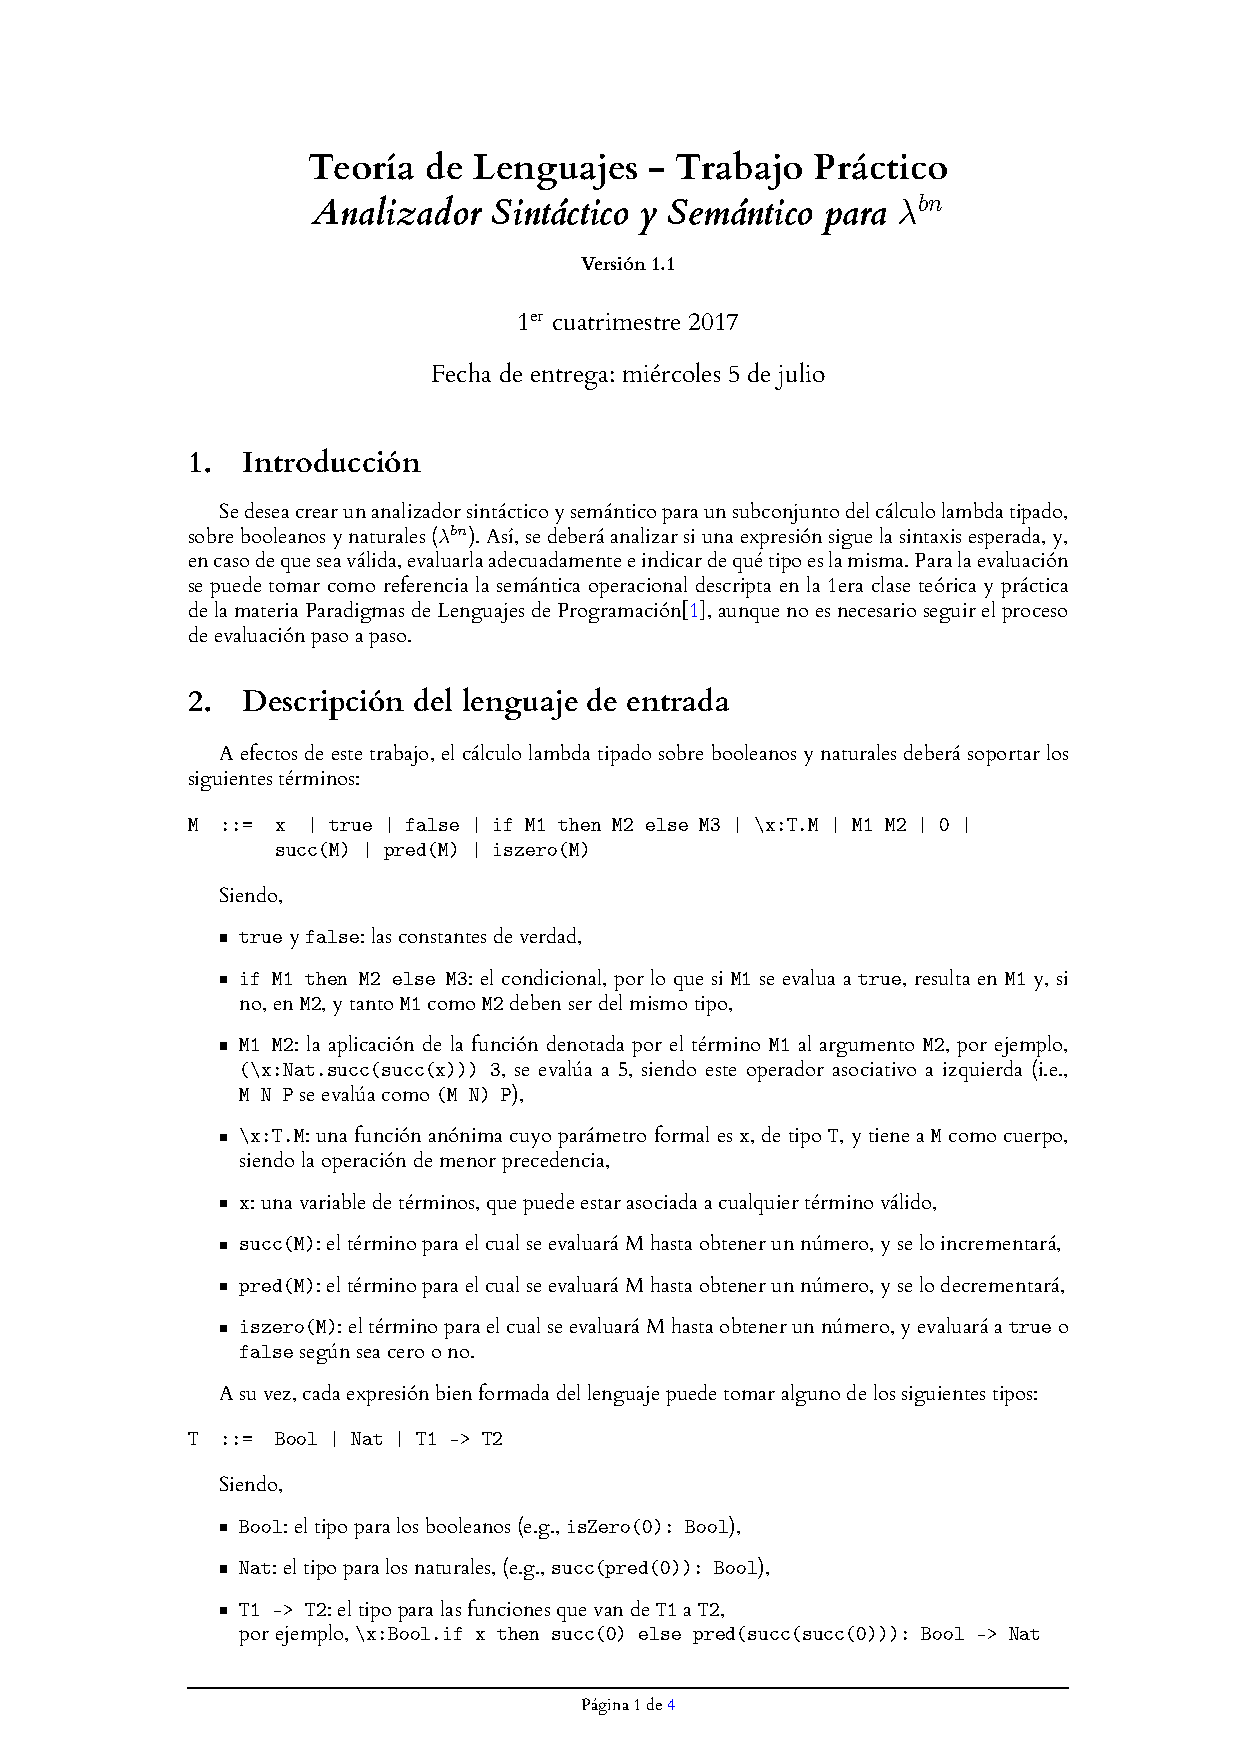
\includepdf[pages={1},pagecommand=\section{Enunciado},offset=40 -75]{enunciado.pdf}
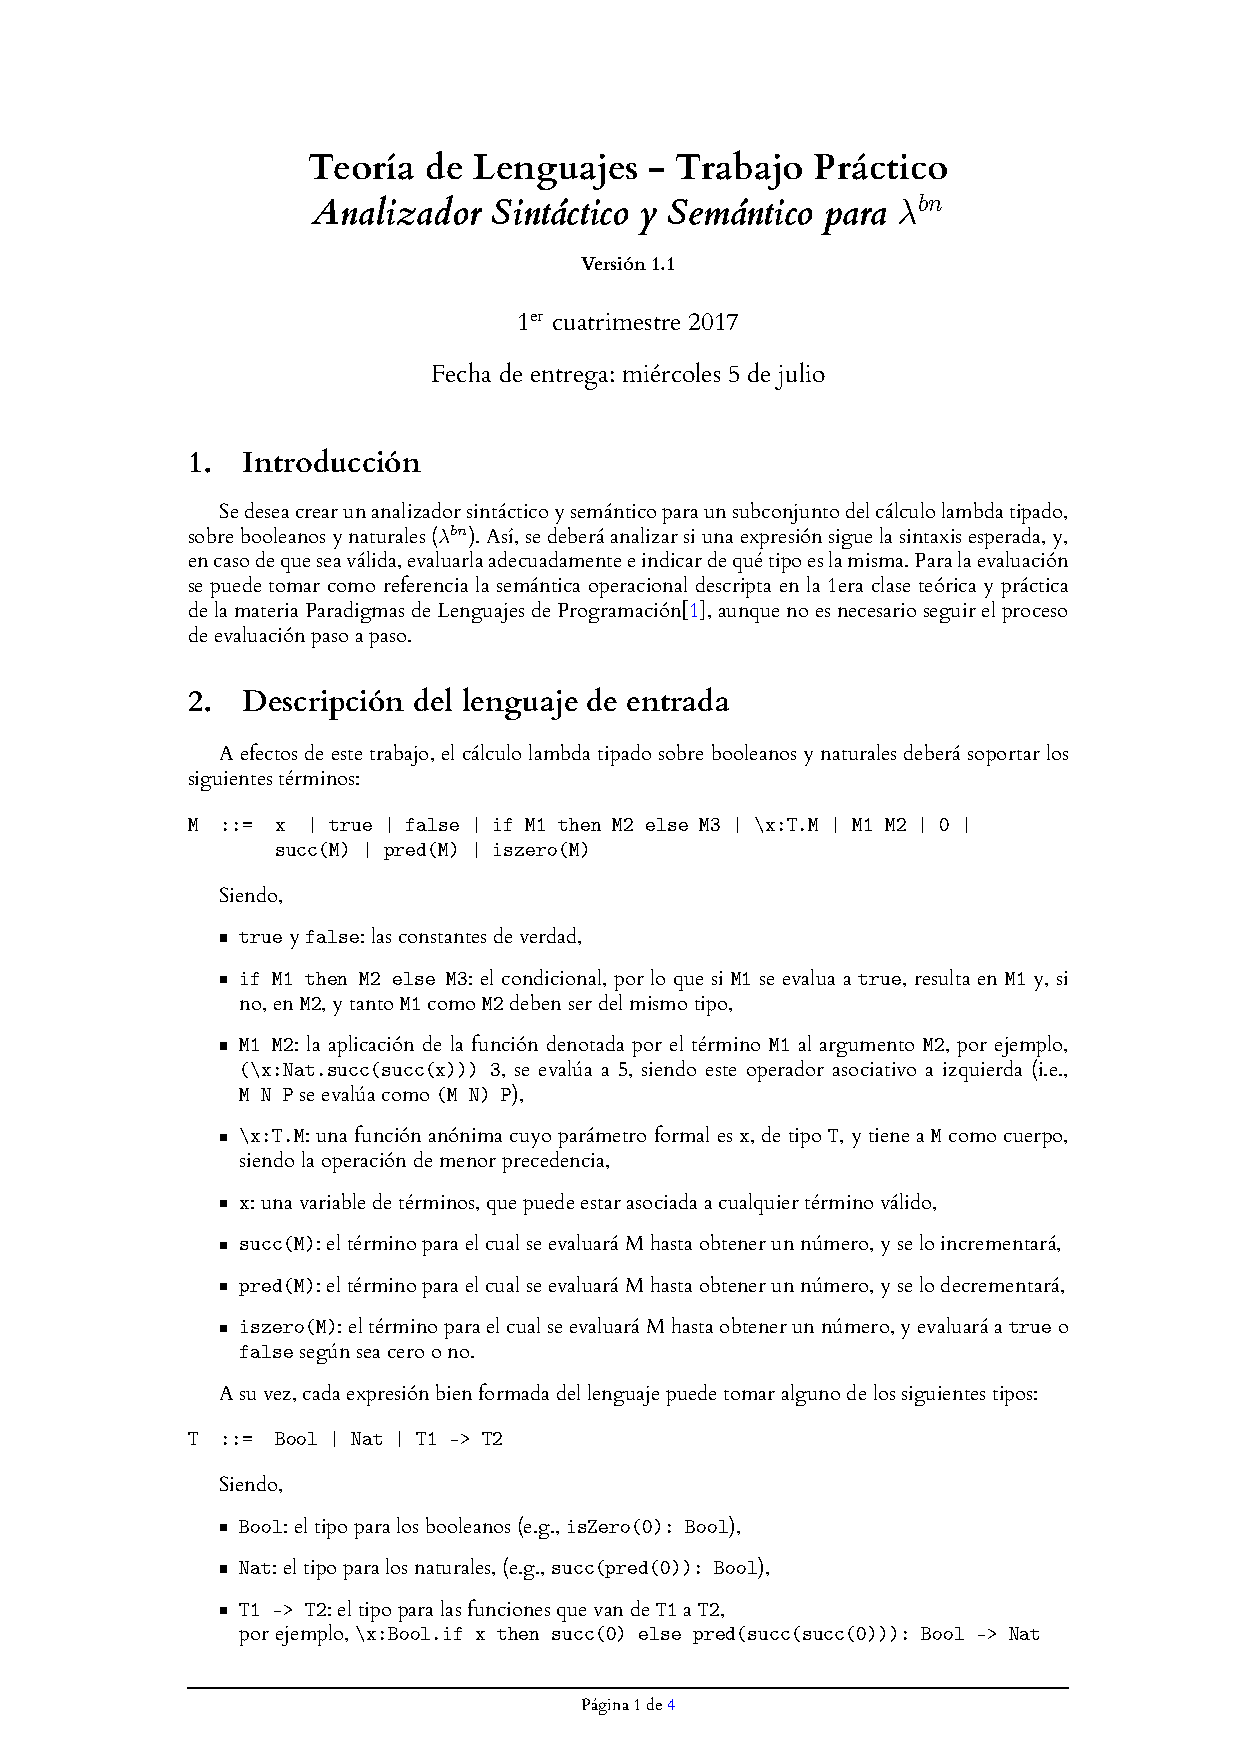
\includepdf[pages={1,2,3,4},offset=40 -75]{enunciado.pdf}

\end{document}
